% 
\documentclass[a4paper]{article}
\usepackage[OT1]{fontenc}
\usepackage{Sweave}
\usepackage{cite}
\usepackage{natbib}
\usepackage{fullpage}
\usepackage{color}
\usepackage{appendix}
\usepackage[utf8x]{inputenc} %prevents some encoding issues in R
\definecolor{darkred}{rgb}{0.545,0,0} 
\definecolor{midnightblue}{rgb}{0.098,0.098,0.439} 
\DefineVerbatimEnvironment{Sinput}{Verbatim}{fontshape=sl,formatcom=\color{midnightblue}}
\DefineVerbatimEnvironment{Soutput}{Verbatim}{fontshape=sl,formatcom=\color{darkred}}
\DefineVerbatimEnvironment{Scode}{Verbatim}{fontshape=sl,formatcom=\color{black}}


\begin{document}

\title{An Exploration of Mixed Effects Random Graph Models}
\author{Jeroen C.L. Ooms}

\maketitle

\abstract{}
An interesting generalization of Exponential Random Graph Models (ERGM) is to model dyad level effects as random effects at the node level. 
This allows for fitting of variances and covariances of well established ergm-terms, which gives insight in both the data and these terms.
This paper is an informal exploration of the possibilities and limitations of this approach. 
The idea is illustrated with examples from some well known datasets that were fit using standard multilevel software.
Results show that there are some interesting questions that can be adressed using this approach, however caution is required as the appropriateness of
including random effects is often problem specific. The code that was used is publicly available in the form of an R package.

\section{Introduction}

The premise of this research is the desire to model individual differences of predictor terms in Exponential Random Graph Models (ERGM). As a basic example, 
we would like to explore differences in individual popularity and activity of people in a network. 
One way to do this is to add a seperate activity/popularity coefficient to the \texttt{ergm} model for every person in the network. 
However, this is not the most elegant solution, because $n$ parameters have to be added to the model for every term, which will lead quickly to overparameritizing the model. 
As a natural alternative, we propose to estimate these terms as random effects on the node-level in a mixed effects model. 
This way between-group variances, and potentially covariances of \texttt{ergm} terms can be modeled to explore how they contribute to predicting the ties in our network. \\

We start the paper with a brief review of mixed models and propose methods for applying them to both directed and undirected networks. 
Section \ref{section.hansell} explains how some of the standard multilevel concepts and practices could apply to random graph models.
Every subsection is illustrated with a basic example from the Hansell dataset.
Section \ref{section.lazega} explores how far we can push this concept on a more complex dataset, using the well known Lazega data. 
Finally, all results from this paper can be reproduced using code from Appendix \ref{appendix.code} and the R package \texttt{lmergm}, introduced in Appendix \ref{appendix.package}.\\

This paper is intended more as an exploration of ideas rather than claim formal results or suggesting any best practices. 
Methods in this paper are mostly limited to directed networks, that were fit using maximum pseudo likelihood so that the problem reduces
to a logistic regression. This makes the examples easy to understand and we can try them using free software.
More research is required to investigate how for example ergm MCMC methods generalize to mixed effect random graphs.

\section{Mixed Effect Models and Random Graphs}

In many social science applications data appears for which the observations are known te belong to observed groups, also called classes. 
When there are reasons to assume that observations within the same class are more similar than observations from different classes, this violates the iid assumption.
If we want to fit a linear model which takes this so called intraclass correlation into account, we need to distinguish variance that arises from individual differences 
from variance due to group membership. Mixed effect models, also called random effect models or multilevel models, are a class of models that facilitates this. \\

\noindent The mixed linear model \citep{de2008handbook} is written as:
$$
y = X \beta + Z \delta + \epsilon
$$
where $X$ and $Z$ are observed, and
$$
\left( \begin{array}{c} \epsilon \\ \delta  \end{array} \right) \sim N \left( \left( \begin{array}{c} 0 \\ 0 \end{array} \right), \left( \begin{array}{cc} \Sigma & 0 \\ 0 & \Omega \end{array} \right) \right)
$$
where it is custom to assume $\Sigma = \sigma I$. Basically, we split the regression part of the model into a component with fixed coefficients and a component with random coefficients, so that:
$$
y \sim N (X \beta, V)
$$ 
with
$$
V = Z \Omega Z' + \Sigma
$$
By introducing random coefficients into the model we can explain some additional variance that is due to the grouping structure of the data.\\

Mixed effects models are most commonly used in settings where the data has an hierarchical structure. For example, common in clinical trials is data where patients are grouped
by the nurse they were treated by, within certain participating hospitals. So this could be modelled as a  3 level structure, with patients 'within' nurses, and nurses within hospitals.
The treatment effect can then be modeled conditional on the hospital and the nurse of the patient:
$$
y_{ijk} = \beta_0 + \beta_1 * \mathrm{treatment} + \nu_k + \upsilon_{jk} + \epsilon_{ijk}
$$
where $\nu_k$ is error variance on the hospital level, $\upsilon_{jk}$ is error variance on the nurse level, and $\epsilon_{ijk}$ is residual variance. If there is an
hypothesis that the effectivity of the treatment will vary between hospitals (e.g. because of size or location), a random coefficient for treatment can be added to the model:
$$
y_{ijk} = \beta_0 + \beta_1 * \mathrm{treatment} + \gamma_{k} * \mathrm{treatment} + \nu_k + \upsilon_{jk} + \epsilon_{ijk}
$$
Although mixed effects models are often associated with hierarchical data, and some software packages always assume levels to be nested, this 
is not at all required. The concept of a mixed model is actually much more general, although for exotic models estimation can get
more complicated, and specialized software and algorithms might be required. \\

One interesting class of mixed models that does not assume hierarchical data are crossed effects models. In a crossed effects model there are at least two
grouping factors, however one is not contained within the other \citep[chapter. 8.2]{de2008handbook}, \citep{browne2001multiple, rasbash1994efficient}. 
An example would be a model in which we do a clinical trial with patiens from several neighborhoods,
which are treated in the experiment by randomly assigned nurses. For this data we could include random effects both on the neighborhood level as well as the
nurse level. \\

Another less well known class of mixed models that is relevant for this paper is known in the literature as the Multi Membership Mixed Model \citep[chapter. 8.3]{de2008handbook}, \citep{browne2001multiple}. 
This model is a straightfoward generalization of a regular mixed model, however we allow for the possebility that an observation might belong to more than one group within the same 
grouping factor. For example, an experiment in which patients are treated by multiple nurses could be modeled using a multi membership mixed model.

  
\subsection{Directed networks as Crossed Effects Mixed Effects Model}

\begin{figure}[h!]
\centering
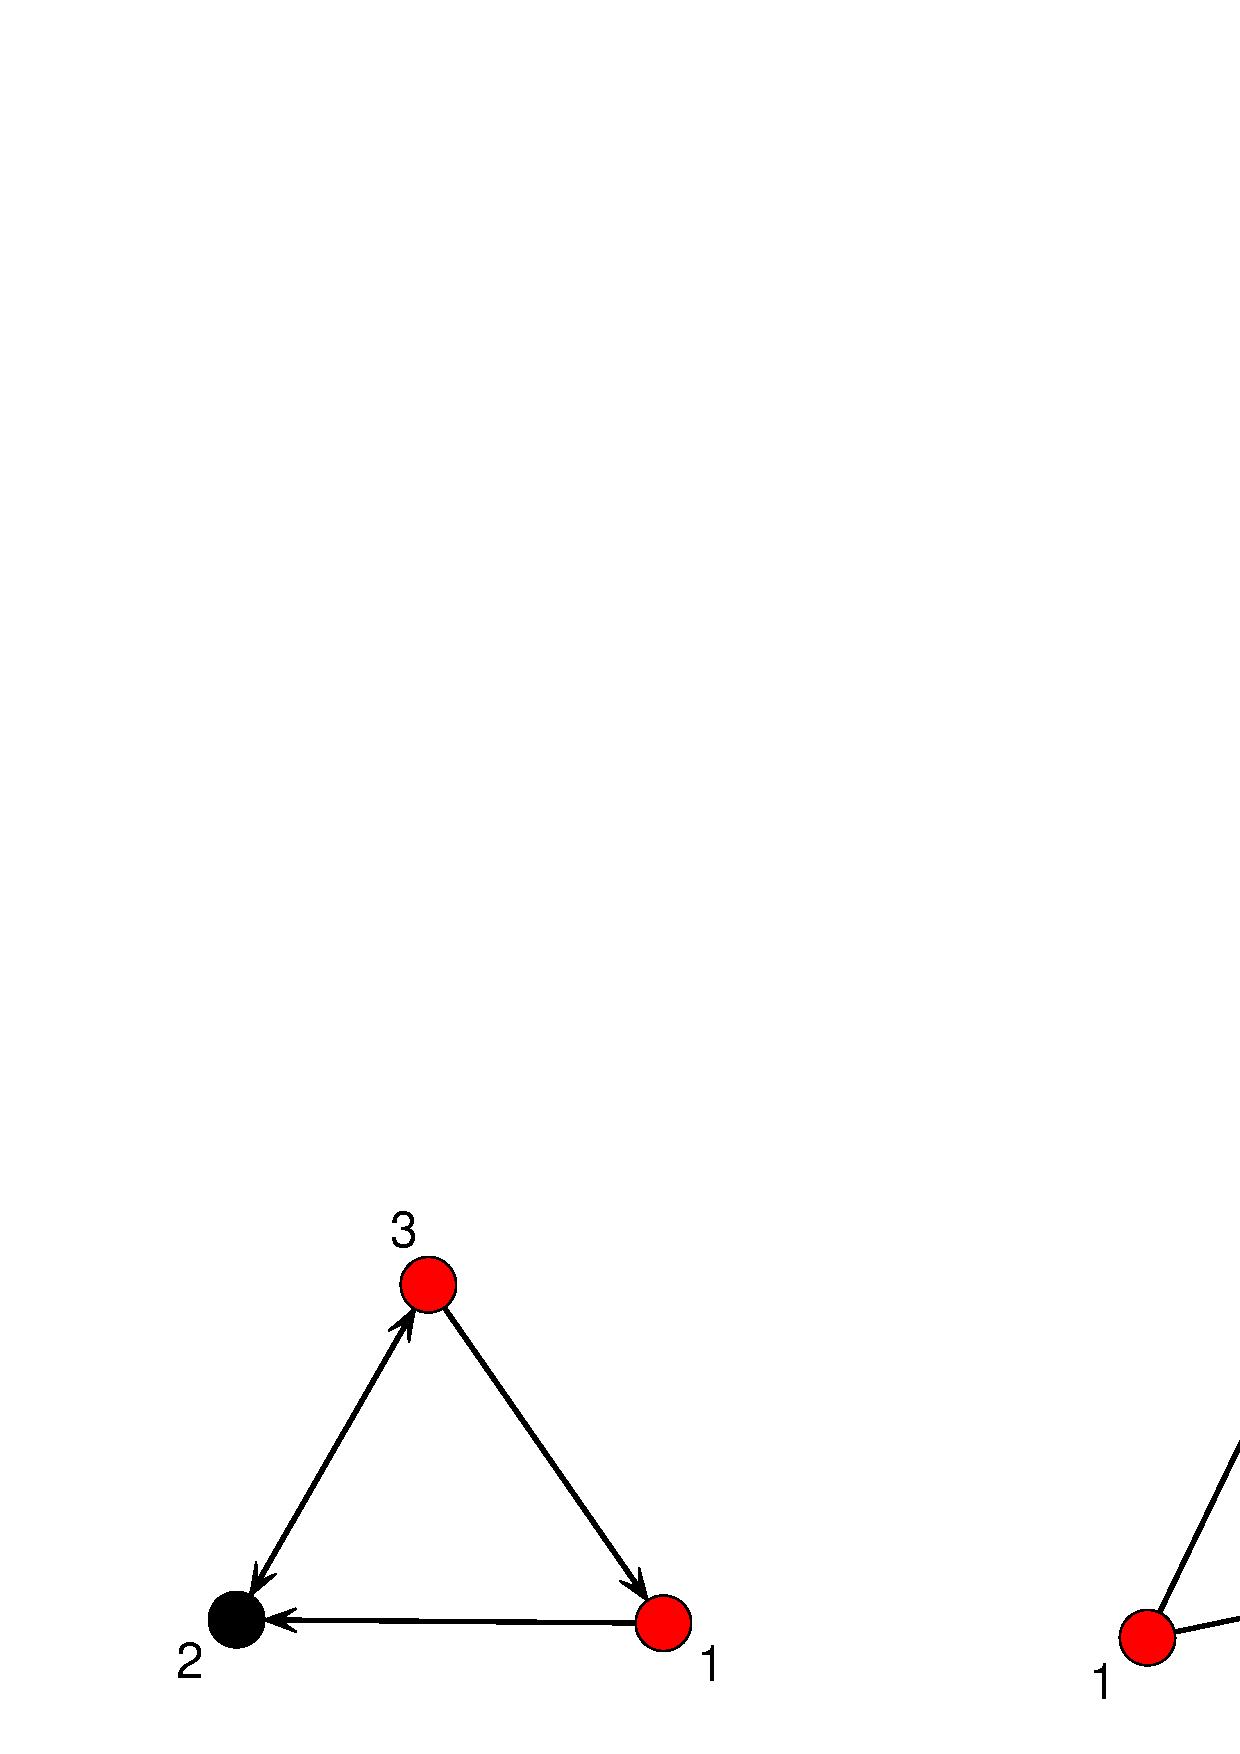
\includegraphics{paper-mininet}
\caption{A simple directed (left) and undirected (right) 3 node network}
\label{fig:mininet1}
\end{figure}

In order to be able to fit a mixed effects model on network data, we need to transform the network into an appropriate design matrix. The shape of the data
is more than an technicallity in this case. It defines what exactly we consider to be the grouping factor, which is not completely trivial. \\

For a directed graph the most straightfoward representation of the data is by completely expanding it into a matrix with one row 
for every possible edge. For example, the left network in \ref{fig:mininet1} shows an example of a tiny 3 node network,
which would be represented as listed in table \ref{minitable}. Once the data is in this form, we can use standard multilevel software
to fit a crossed effect model with a random effect on the sender and a random effect on the receiver level. 


% latex table generated in R 2.12.1 by xtable 1.5-6 package
% Sun Jun 12 15:00:04 2011
\begin{table}[ht]
\begin{center}
\begin{tabular}{rrrrrr}
  \hline
 & y & nodematch.sex & transitiveties & receiver & sender \\ 
  \hline
1 & 1 & 0 & 1 & 2 & 3 \\ 
  2 & 1 & 0 & 1 & 2 & 1 \\ 
  3 & 0 & 1 & 2 & 3 & 1 \\ 
  4 & 0 & 0 & 2 & 1 & 2 \\ 
  5 & 1 & 1 & 1 & 1 & 3 \\ 
  6 & 1 & 0 & 0 & 3 & 2 \\ 
   \hline
\end{tabular}
\caption{Full expansion of the directed 3 node network.}
\label{minitable}
\end{center}
\end{table}
This is a fairly straightforward approach, and we will use this model in our examples throughout the paper. However, notice that we made
some choices here. By modelling this as a crossed effects model, we are not taking into account that the sender and receiver are of the same grouping factor.
Hence, we cannot include for example a covariance between a popularity and activity term. 

\subsection{Undirected networks as Multi Membership Mixed Effects Model}

For undirected networks a crossed effects model is not possible, because there is no order in the two nodes that belong to an edge.
Instead we can use a Multi Membership Mixed Model, with only one random effect group (node) which has two members.
Table \ref{minitable2} shows an example of the covariates matrix of the undirected three node network depicted in the right plot in figure \ref{fig:mininet1}.
The table has 2 columns both called node, to emphasize that these are two members of one and the same grouping factor.

% latex table generated in R 2.12.1 by xtable 1.5-6 package
% Sun Jun 12 15:00:04 2011
\begin{table}[ht]
\begin{center}
\begin{tabular}{rrrrr}
  \hline
 & y & nodematch.sex & node & node \\ 
  \hline
6 & 0 & 0 & 1 & 2 \\ 
  4 & 1 & 1 & 1 & 3 \\ 
  3 & 1 & 0 & 2 & 3 \\ 
   \hline
\end{tabular}
\caption{Full expansion of an undirected 3 node network.}
\label{minitable2}
\end{center}
\end{table}
This research primarely focuses on the directed case. Two reasons for this are that the undirected case is in many ways a simplified 
version of the directed case. On top of that, a practical reason was that specialized software would be needed to fit multi membership
mixed models, whereas crossed effect mixed models can be fitted using the open source R package \texttt{lme4} \citep{bates2007lme4, rmanual}.

\section{Some basic examples using Hansell data}
\label{section.hansell}

This section illustrates how some common multilevel concepts and practices can be applied to mixed effect random graph models. 
Every subsection is illustrated with a example from the Hansell dataset. 
This is a network of strong friendship ties among 13 boys and 14 girls in a sixth-grade classroom, as collected by \citet{hansell1984cooperative} and reported by \citet{wang1987stochastic}.
It is a directed graph with only one vertex attribute (gender), and therefore it makes nice simple examples. Figure \ref{fig:hansellplot} shows a
plot of the data.

\begin{figure}[h!]
\centering
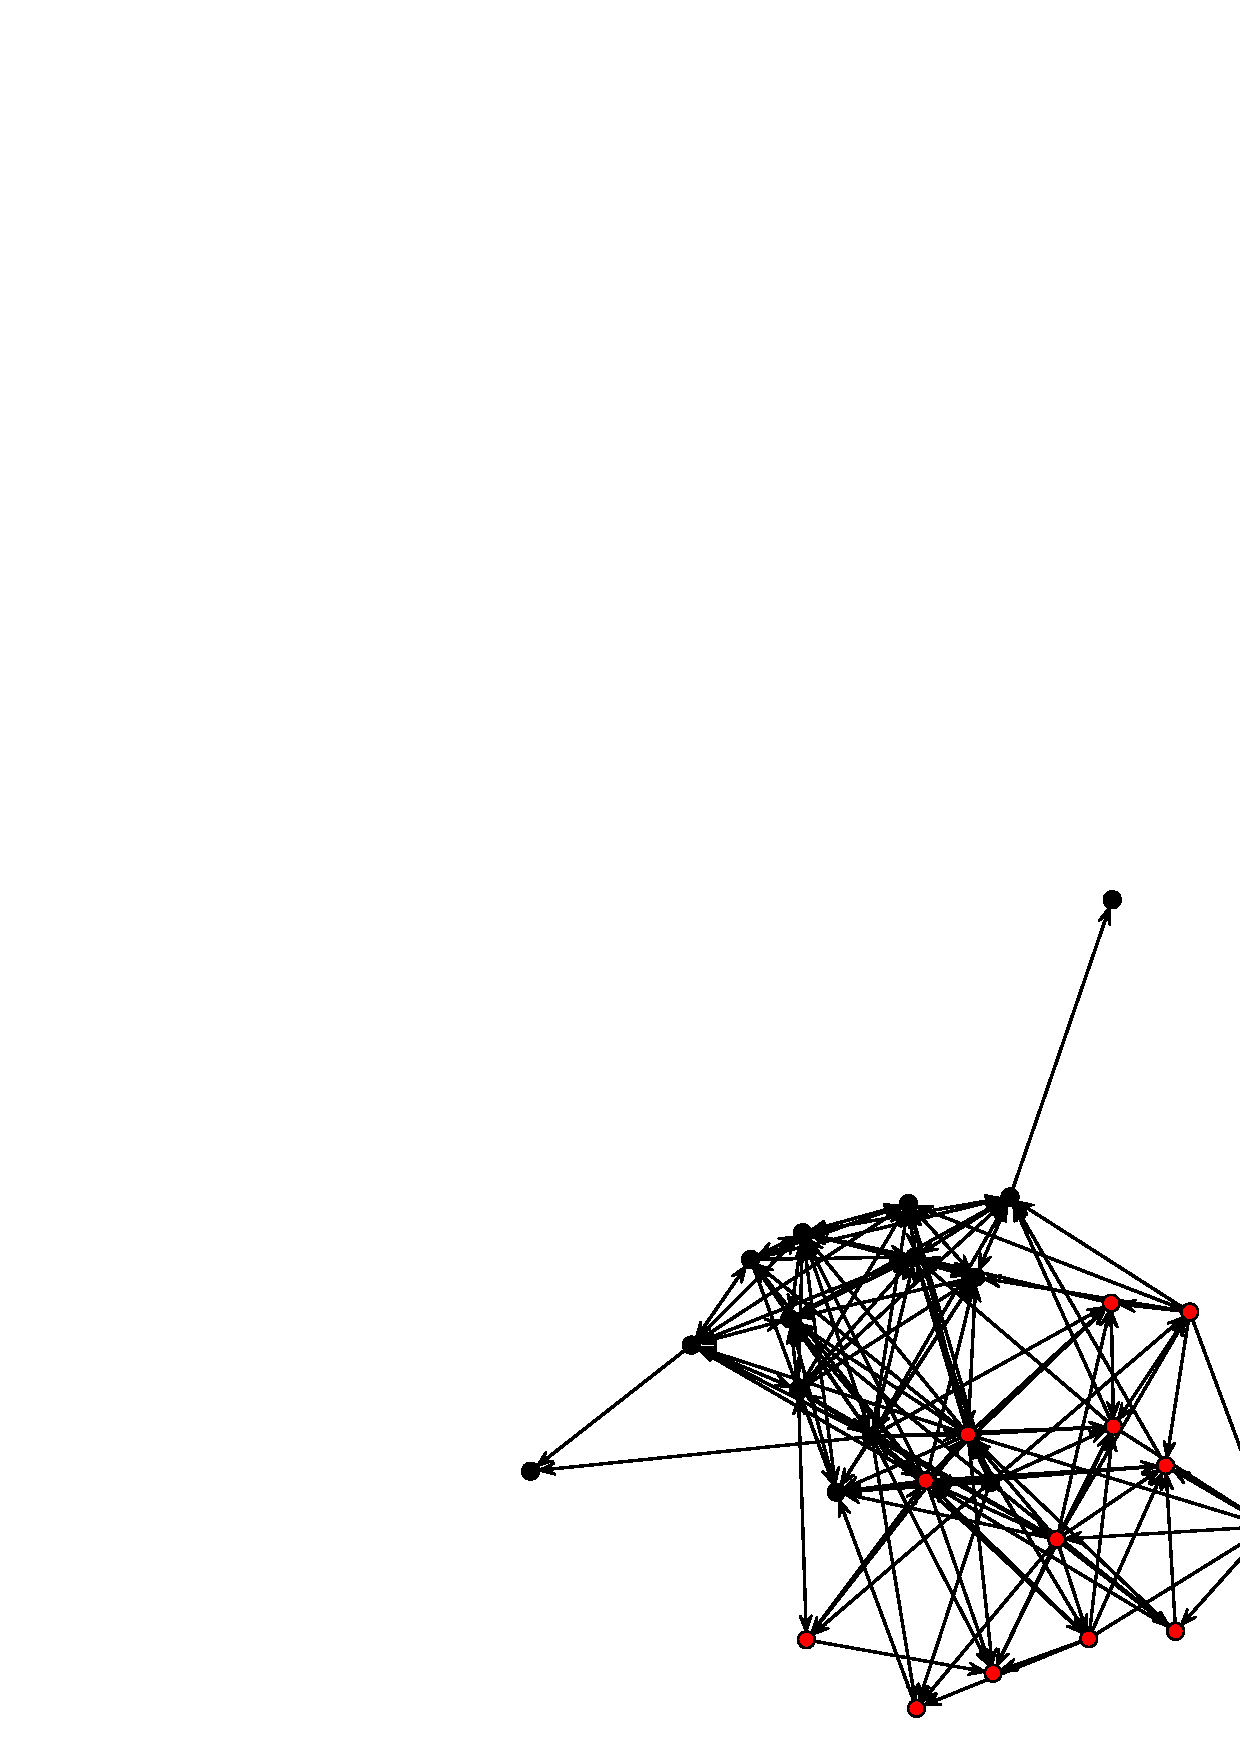
\includegraphics{paper-hansellplot}
\caption{Plot of the hansell data}
\label{fig:hansellplot}
\end{figure}


\subsection{The \texttt{lmergm} package and the model formula}

All of the models that will be presented in this paper can be reproduced using functions that have 
been implemented in the \texttt{lmergm} package. The \texttt{lmergm} package depends on the \texttt{lme4} \citep{bates2007lme4} and \texttt{ergm} \citep{hunter2008ergm} packages.
It uses social network terms that are available in \texttt{ergm} to build a covariates matrix that is then
dispatched to \texttt{lme4} to define and fit a multilevel model. 
Details about the package have been moved to Appendix \ref{appendix.package}\\

One thing that is important to understand in advance though is the \texttt{lmergm} model \emph{formula}. Both \texttt{ergm} and \texttt{lme4}
use an R formula to specify the model. In the \texttt{lmergm} package one also needs to specify the model using
a formula, which is a mix of the \texttt{lme4} and \texttt{ergm} syntax. Random effects in \texttt{lme4} are specified by including
a term that contains a vertical bar. In \texttt{lmergm} two random effect groups can be specified: \texttt{sender} and \texttt{receiver}.
Hence a formula could look like this:
\begin{Schunk}
\begin{Soutput}
hansell ~ edges + match("sex") + (edges + match("sex") | sender)
\end{Soutput}
\end{Schunk}
This formula specifies an \texttt{ergm} model with an intercept and a homophily term that are random on the sender level. 
Note that it is usually wise to include a fixed effect for any random effect, unless we have reasons to assume the effect has been centered already.
Also by default \texttt{lme4} includes covariance random effects if there are more than 1 random effect specified within
the same term. Hence the formula above will fit 2 fixed and 3 random coefficients. 


\subsection{Distribution and Shrinkage of Coefficients}

We start out by exploring how random the coefficiens are in the first place. One thing we can do is initially
fit a regular \texttt{ergm} model in which we include seperate activity and popularity coefficients for every person, 
and look at the distribution of MLE estimates, as done in figure \ref{fig:coefhist}.
\begin{Schunk}
\begin{Sinput}
> hansell.ca1 <- ergm(hansell ~ receiver(0))
> hansell.ca2 <- ergm(hansell ~ sender(0))
> par(mfrow = c(1, 2))
> hist(coef(hansell.ca1), main = "receiver", xlab = "mle")
> hist(coef(hansell.ca2), main = "sender", xlab = "mle")
\end{Sinput}
\end{Schunk}
\begin{figure}[h!]
\centering
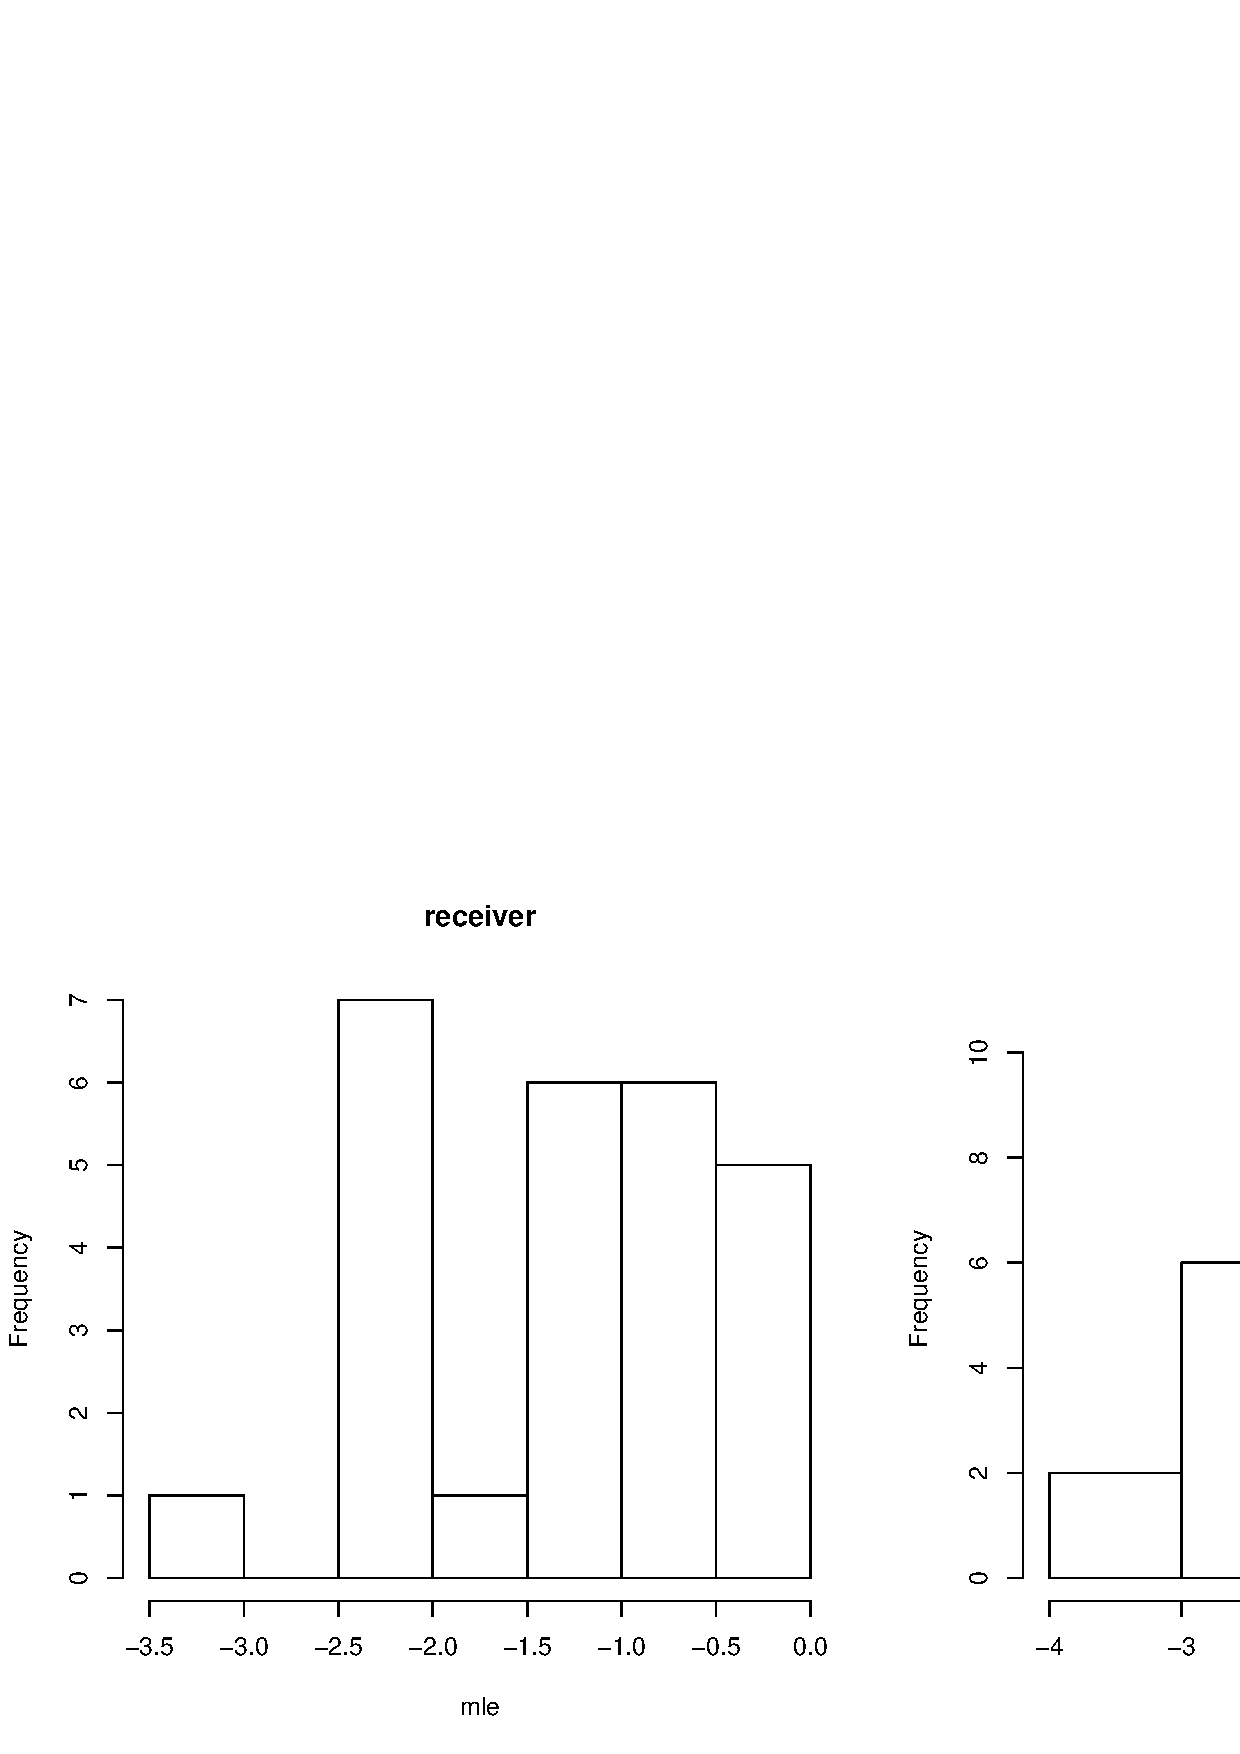
\includegraphics{paper-coefhist}
\caption{Distributions of the popularity and activity coefficients}
\label{fig:coefhist}
\end{figure}

We notice that the MLE's of the coefficients are definely not perfectly normal, but things could have been worse. 
Both the popularity (receiver dummies) and activity (sender dummies) coefficients shows some skewness towards the right with a tail on the left. 
Also note that some coefficients were estimated by ergm at $-\infty$ and have not been included in the histogram. \\

Even though the empirical distribution of the coefficient MLE's under a fully parametrized \texttt{ergm} model is not perfectly normal, 
this does not necessarily mean that modeling these coefficients as Guassian distributed gives us very misleading results. 
It might even beneficial to some extend: by assuming a normal distribution, the coeffients "borrow information" from each other
and we could we could obtain some useful shrinkage. This idea goes back to \citet{james1961estimation} who show that Stein's estimator
has a uniformly lower MSE than the MLE for estimating the mean of a Guassian distribution. 
Similar reasoning motivates Bayesian Hierarchical models \citep{gelman2004bayesian}. \\

For example in the ergm model, individual popularity coefficients are estimated at $-\infty$ when a persons did not receive any
ties in this particular dataset. However, one could argue that the MLE of $-\infty$, corresponding to a probability of this person ever
receiving a tie being equal to $0$ is too extreme, as it is not completely unthinkable that these persons would receive some ties 
under repititions of the social process underlying this network. It might make more sense to look at the distribution of receiving ties
among all nodes in the network, and put these persons in the lower end of the distribution rather than all the way at $-\infty$.  \\

To explore how this could work out in a real dataset, mixed effect random graph models with equivalent parametrization as the ergm models 
were fit in order to be able to compare the MLE coefficients to the best linear unbiased predictors (blup) of these coefficients 
under the analogous mixed effects model. 
 
\begin{Schunk}
\begin{Sinput}
> hansell.cb1 <- lmergm(hansell ~ edges + (1 | receiver))
> hansell.cb2 <- lmergm(hansell ~ edges + (1 | sender))
> par(mfrow = c(1, 2))
> plot(coef(hansell.ca1), coef(hansell.cb1)$receiver[[1]], main = "receiver", 
+     xlab = "Fixed coefficients", ylab = "Random BLUPS", xlim = c(-3, 
+         1), ylim = c(-3, 1))
> abline(0, 1, col = "red")
> plot(coef(hansell.ca2), coef(hansell.cb2)$sender[[1]], main = "sender", 
+     xlab = "Fixed coefficients", ylab = "Random BLUPS", xlim = c(-3, 
+         1), ylim = c(-3, 1))
> abline(0, 1, col = "red")
\end{Sinput}
\end{Schunk}
\begin{figure}[h!]
\centering
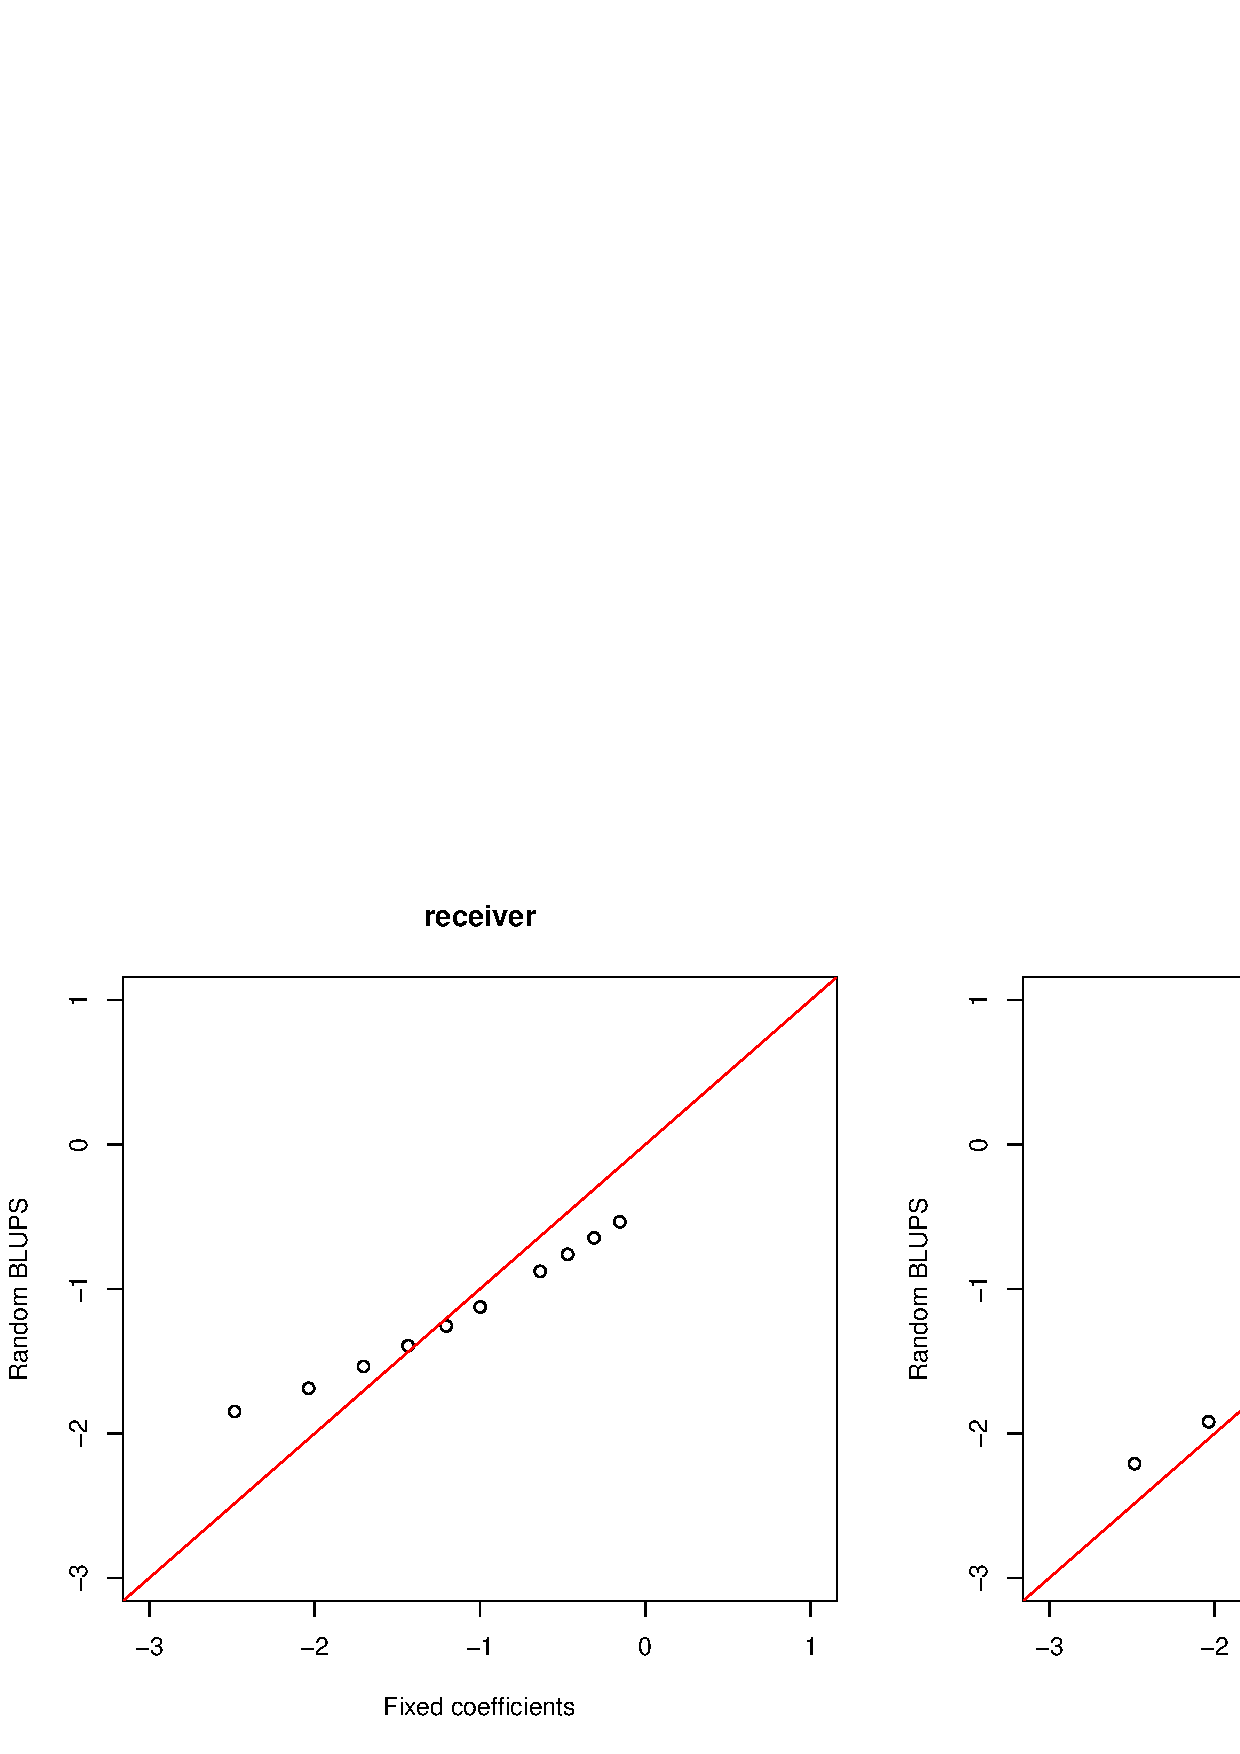
\includegraphics{paper-comparecoef}
\caption{Comparison of popularity and activity MLE's and Mixed Model BLUPs. Red line is the identity.}
\label{fig:comparecoef}
\end{figure}

% latex table generated in R 2.12.1 by xtable 1.5-6 package
% Sun Jun 12 15:00:06 2011
\begin{table}[ht]
\begin{center}
\begin{tabular}{lrrrr}
  \hline
 & popularity.fixed & popularity.random & activity.fixed & activity.random \\ 
  \hline
node 1 & -1.00 & -1.12 & -1.20 & -1.26 \\ 
  node 2 & -1.20 & -1.26 & -2.48 & -2.21 \\ 
  node 3 & -2.04 & -1.69 & -1.00 & -1.08 \\ 
  node 4 & -2.04 & -1.69 & -0.15 & -0.31 \\ 
  node 5 & -1.00 & -1.12 & -0.00 & -0.18 \\ 
  node 6 & -1.00 & -1.12 & -0.47 & -0.60 \\ 
  node 7 & -2.04 & -1.69 & -1.70 & -1.67 \\ 
  node 8 & -2.48 & -1.85 & -1.00 & -1.08 \\ 
  node 9 & -1.20 & -1.26 & -2.04 & -1.92 \\ 
  node 10 & -1.00 & -1.12 & -Inf & -3.00 \\ 
  node 11 & -1.70 & -1.54 & -3.22 & -2.56 \\ 
  node 12 & -2.04 & -1.69 & -2.04 & -1.92 \\ 
  node 13 & -1.20 & -1.26 & -2.48 & -2.21 \\ 
  node 14 & -0.64 & -0.88 & -1.00 & -1.08 \\ 
  node 15 & -0.15 & -0.53 & -1.44 & -1.45 \\ 
  node 16 & -1.44 & -1.39 & 1.00 & 0.66 \\ 
  node 17 & -0.31 & -0.65 & -3.22 & -2.56 \\ 
  node 18 & -0.47 & -0.76 & -2.48 & -2.21 \\ 
  node 19 & -2.04 & -1.69 & -0.31 & -0.45 \\ 
  node 20 & -Inf & -2.20 & -0.31 & -0.45 \\ 
  node 21 & -0.47 & -0.76 & -1.44 & -1.45 \\ 
  node 22 & -1.20 & -1.26 & -0.81 & -0.91 \\ 
  node 23 & -1.44 & -1.39 & -1.00 & -1.08 \\ 
  node 24 & -0.64 & -0.88 & -2.04 & -1.92 \\ 
  node 25 & -0.47 & -0.76 & -0.81 & -0.91 \\ 
  node 26 & -3.22 & -2.02 & -Inf & -3.00 \\ 
  node 27 & -2.48 & -1.85 & -Inf & -3.00 \\ 
   \hline
\end{tabular}
\caption{Fixed effect MLE's and random effect BLUPs of popularity and activity}
\label{coeftable}
\end{center}
\end{table}
Figure \ref{fig:comparecoef} shows the plots that compares the fixed effect MLE's with the BLUPs under the mixed effect models. The red line denotes the identity line.
We observe exactly what we would have expected: the fixed effects are shrunk towards the mean in the random effects model. And even though
the distribution of the fixed effects was not perfectly normal, nothing unexpected seems to be happening, at least judging from these pictures.
We do note that the popularity coefficients have had some more shrinkage than the activity coefficients, probably because their distribution 
was somewhat less normal.
In addition, table \ref{coeftable} shows the same data, and we can see that the MLE's that were $-\infty$ have been shrunk towards $-2.20$ and $-3.00$
for respectively the popularity and activity coefficient. If we would draw a line through the points in figure \ref{fig:comparecoef}, 
these values would correspond to the left asymptote.



 



\subsection{The Fixed Effects only \texttt{ergm} models}

Suppose we are interested in patterns of homophily and transitivity in our network. We write the \texttt{ergm} model like this:
$$
logit(y) = \beta_0 + \beta_1 * \mathrm{transitive} + \beta_2 * \mathrm{match.sex}
$$
Let's start by fitting a standard \texttt{ergm} model that fits fixed effects for $\beta_0, \beta_1, \beta_2$. we call this model $M0$. 
Because this model does not contain any random effects yet, it can be fit using the \texttt{ergm} package. The following code was used: 
\begin{Schunk}
\begin{Sinput}
> hansell.0 <- ergm(hansell ~ edges + transitiveties + match("sex"), 
+     MPLEonly = T)
> summary(hansell.0)
\end{Sinput}
\begin{Soutput}
==========================
Summary of model fit
==========================

Formula:   hansell ~ edges + transitiveties + match("sex")

Newton-Raphson iterations:  5 

Maximum Pseudolikelihood Results:
               Estimate Std. Error MCMC s.e. p-value    
edges           -2.2661     0.1921        NA < 1e-04 ***
transitiveties   0.3206     0.1090        NA 0.00338 ** 
nodematch.sex    1.1995     0.2009        NA < 1e-04 ***
---
Signif. codes:  0 ‘***’ 0.001 ‘**’ 0.01 ‘*’ 0.05 ‘.’ 0.1 ‘ ’ 1 

Warning:  The standard errors are based on naive pseudolikelihood and are suspect.

    Null  Pseudo-deviance: 973.18  on 702  degrees of freedom
 Residual Pseudo-deviance: 690.56  on 699  degrees of freedom
          Pseudo-deviance: 282.62  on   3  degrees of freedom
 
AIC: 696.56    BIC: 710.22 
\end{Soutput}
\end{Schunk}
The first column in Table \ref{hansellcoef} shows the fitted coefficients for this model. 
All fixed effects were found to be significant in this model, and based on this model we would conclude that the network shows evidence for both
gender based homophily and transitivity. \\  


\subsection{Adding Random Intercepts}

In our next model ($M1$), a random intercept on both the sender and the receiver level was added. These could be interpreted as 
random coefficients for the activity and popularity of individual children in the network. The model was fit using: 
\begin{Schunk}
\begin{Sinput}
> hansell.1 <- lmergm(hansell ~ edges + transitiveties + match("sex") + 
+     (edges | sender) + (edges | receiver))
> summary(hansell.1)
\end{Sinput}
\begin{Soutput}
Generalized linear mixed model fit by the Laplace approximation 
Formula: y ~ 1 + transitiveties + nodematch.sex + (1 | sender) + (1 |      receiver) 
   Data: cmatrix 
   AIC   BIC logLik deviance
 613.4 636.2 -301.7    603.4
Random effects:
 Groups   Name        Variance Std.Dev.
 sender   (Intercept) 1.92777  1.38844 
 receiver (Intercept) 0.81168  0.90093 
Number of obs: 702, groups: sender, 27; receiver, 27

Fixed effects:
                Estimate Std. Error z value Pr(>|z|)    
(Intercept)    -2.795765   0.401142  -6.970 3.18e-12 ***
transitiveties  0.003346   0.152933   0.022    0.983    
nodematch.sex   1.755812   0.239217   7.340 2.14e-13 ***
---
Signif. codes:  0 ‘***’ 0.001 ‘**’ 0.01 ‘*’ 0.05 ‘.’ 0.1 ‘ ’ 1 

Correlation of Fixed Effects:
            (Intr) trnstv
transitivts -0.331       
nodemtch.sx -0.330 -0.206
\end{Soutput}
\end{Schunk}
The results are shown in the second column of Table \ref{hansellcoef}. The terms $\upsilon_0$ and $\nu_0$ reported in the table reflect the variance 
estimates of the random intercept in respectively the senders or receivers. Hence we assume that the popularity (logit probability 
of receiving a tie) is distributed as $N(\beta_0, \nu_0)$ and activity (logit probability of sending a tie) is distributed as 
$N(\beta_0, \upsilon_0)$. \\

% latex table generated in R 2.12.1 by xtable 1.5-6 package
% Sun Jun 12 15:00:09 2011
\begin{table}[ht]
\begin{center}
\begin{tabular}{lrrr}
  \hline
 & M0 & M1 & M2 \\ 
  \hline
$\beta_0$ & -2.27 & -2.80 & -3.22 \\ 
  $\beta_1$ & 0.32 & 0.00 & -0.05 \\ 
  $\beta_2$ & 1.20 & 1.76 & 2.08 \\ 
   \hline
$\upsilon_0$ &  & 1.93 & 3.71 \\ 
  $\upsilon_2$ &  &  & 3.67 \\ 
  $\upsilon_{02}$ &  &  & -2.22 \\ 
  $\nu_0$ &  & 0.81 & 0.55 \\ 
  $\nu_2$ &  &  & 0.46 \\ 
  $\nu_{02}$ &  &  & 0.21 \\ 
   \hline
AIC & 696.56 & 613.39 & 593.63 \\ 
  BIC & 710.22 & 636.16 & 634.61 \\ 
  Deviance & 690.56 & 603.39 & 575.63 \\ 
   \hline
\end{tabular}
\caption{Model Coefficients for Hansell data.}
\label{hansellcoef}
\end{center}
\end{table}
There are some interesting observations here. There is more variance in activity ($\upsilon_0$) of the children than in
their popularity ($\nu_0$). This directly corresponds to the variance in indegree and outdegree of the data nodes.
Additionaly, the fixed effect of transitiveties that was significant on the 0.01 level in model $M0$ has completely vanished 
in $M1$ now that we are controlling for variance in popularity and activity in the model. This shows that there is no 
evidence for transitivity beyond what can be explained by variation in popularity and activity. \\

This finding teaches us something about this dataset, but also about the meaning of transitivity. If shows that observing 
a high number of transitive triads is not necessarily strong evidence for a transitive socialization process. It might was well be an 
artefact of other properties of our data, for example high variation in indegrees and outdegrees. \\

\subsection{Random Slopes and Covariances}

We decide to fit a final model, $M2$, in which also the homophily coefficient has been made random. When there are 2
random effects on both the receiver and sender level, by default also their covariance terms are included.
\begin{Schunk}
\begin{Sinput}
> hansell.2 <- lmergm(hansell ~ edges + transitiveties + match("sex") + 
+     (edges + match("sex") | sender) + (edges + match("sex") | 
+     receiver))
> summary(hansell.2)
\end{Sinput}
\begin{Soutput}
Generalized linear mixed model fit by the Laplace approximation 
Formula: y ~ 1 + transitiveties + nodematch.sex + (1 + nodematch.sex |      sender) + (1 + nodematch.sex | receiver) 
   Data: cmatrix 
   AIC   BIC logLik deviance
 593.6 634.6 -287.8    575.6
Random effects:
 Groups   Name          Variance Std.Dev. Corr   
 sender   (Intercept)   3.71219  1.92670         
          nodematch.sex 3.66738  1.91504  -0.603 
 receiver (Intercept)   0.54871  0.74075         
          nodematch.sex 0.46412  0.68127  0.413  
Number of obs: 702, groups: sender, 27; receiver, 27

Fixed effects:
               Estimate Std. Error z value Pr(>|z|)    
(Intercept)    -3.21879    0.50166  -6.416 1.40e-10 ***
transitiveties -0.04646    0.16308  -0.285    0.776    
nodematch.sex   2.08130    0.50073   4.157 3.23e-05 ***
---
Signif. codes:  0 ‘***’ 0.001 ‘**’ 0.01 ‘*’ 0.05 ‘.’ 0.1 ‘ ’ 1 

Correlation of Fixed Effects:
            (Intr) trnstv
transitivts -0.285       
nodemtch.sx -0.554 -0.104
\end{Soutput}
\end{Schunk}
The third column in Table \ref{hansellcoef} lists the estimated coefficients for this new model.

\subsection{Covariance between random effects}

One thing that we can do naturally using Mixed Effect models is explore the relation between random terms. Figure \ref{ranefplotfig} shows
a scatter plot of the random effect coefficients within the sender and receiver groups in Model 2.  

\begin{Schunk}
\begin{Sinput}
> par(mfrow = c(1, 2))
> plot(ranef(hansell.2)$sender, main = "Sender", xlab = "homophily", 
+     ylab = "activity")
> plot(ranef(hansell.2)$receiver, main = "Receiver", xlab = "homophily", 
+     ylab = "popularity")
\end{Sinput}
\end{Schunk}
\begin{figure}[h!]
\centering
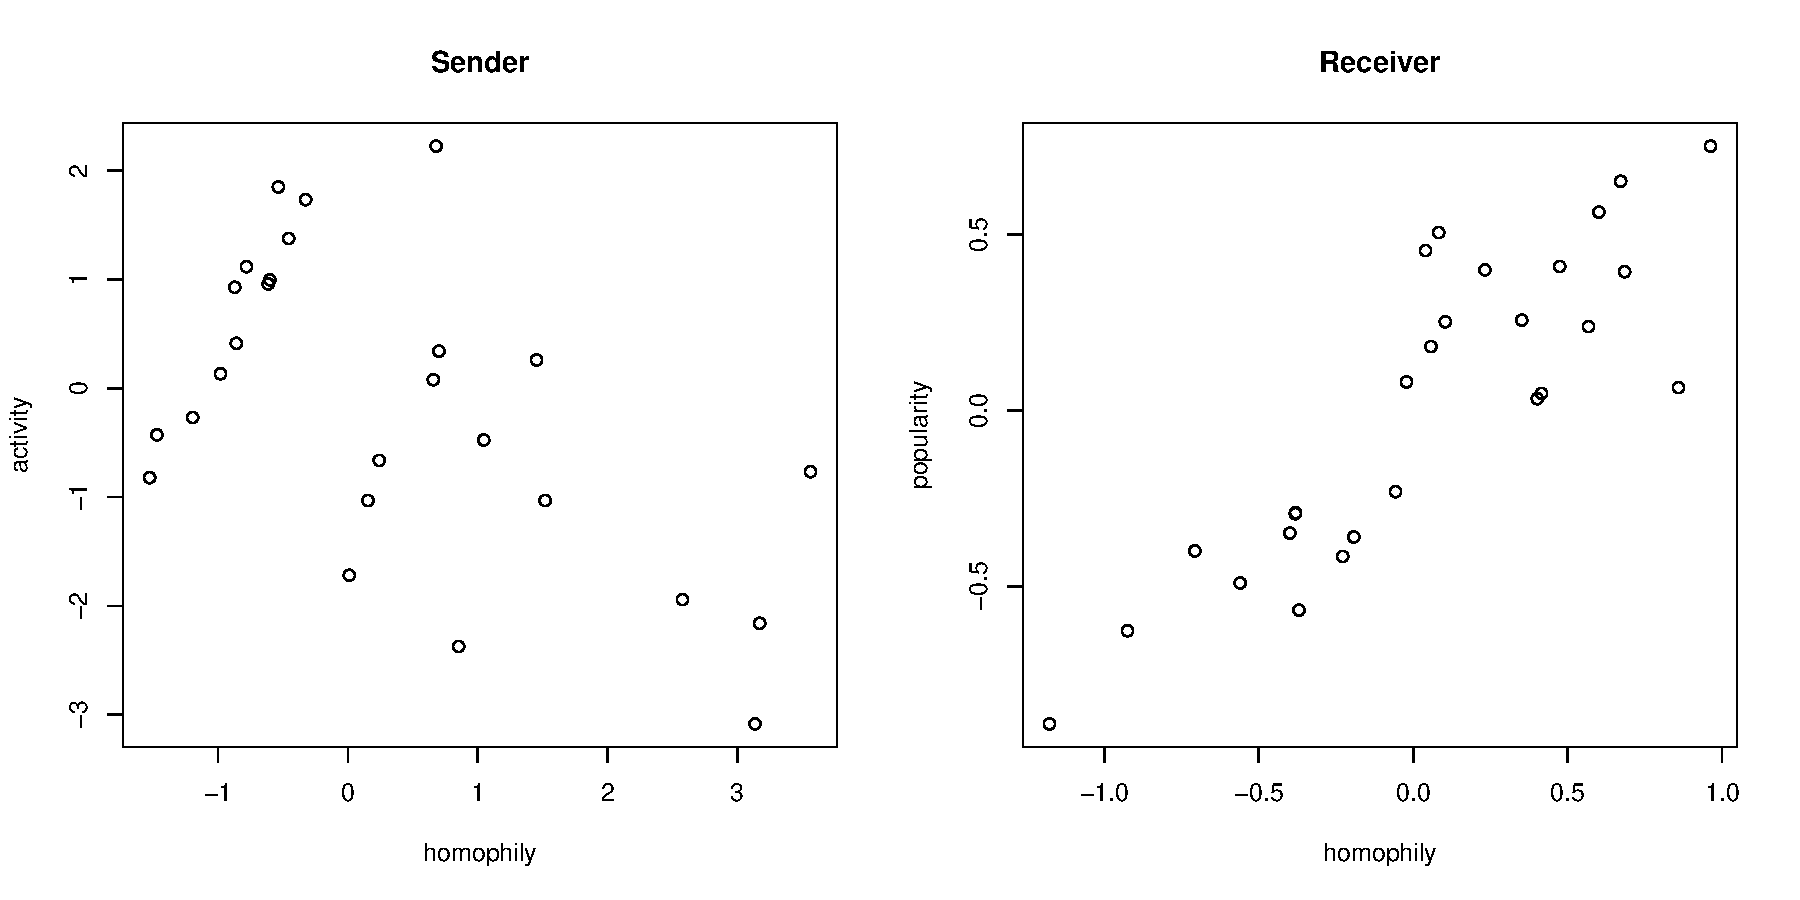
\includegraphics{paper-ranefplotfig}
\caption{Plot of the random effect estimates under model M2.}
\label{ranefplotfig}
\end{figure}
We observe an interesting pattern in which persons that are very active behave less homophilous. However, people that are very popular
mostly seem to be receiving ties, those incoming ties are mostly homophilous ties. \\

\begin{figure}[h!]
\centering
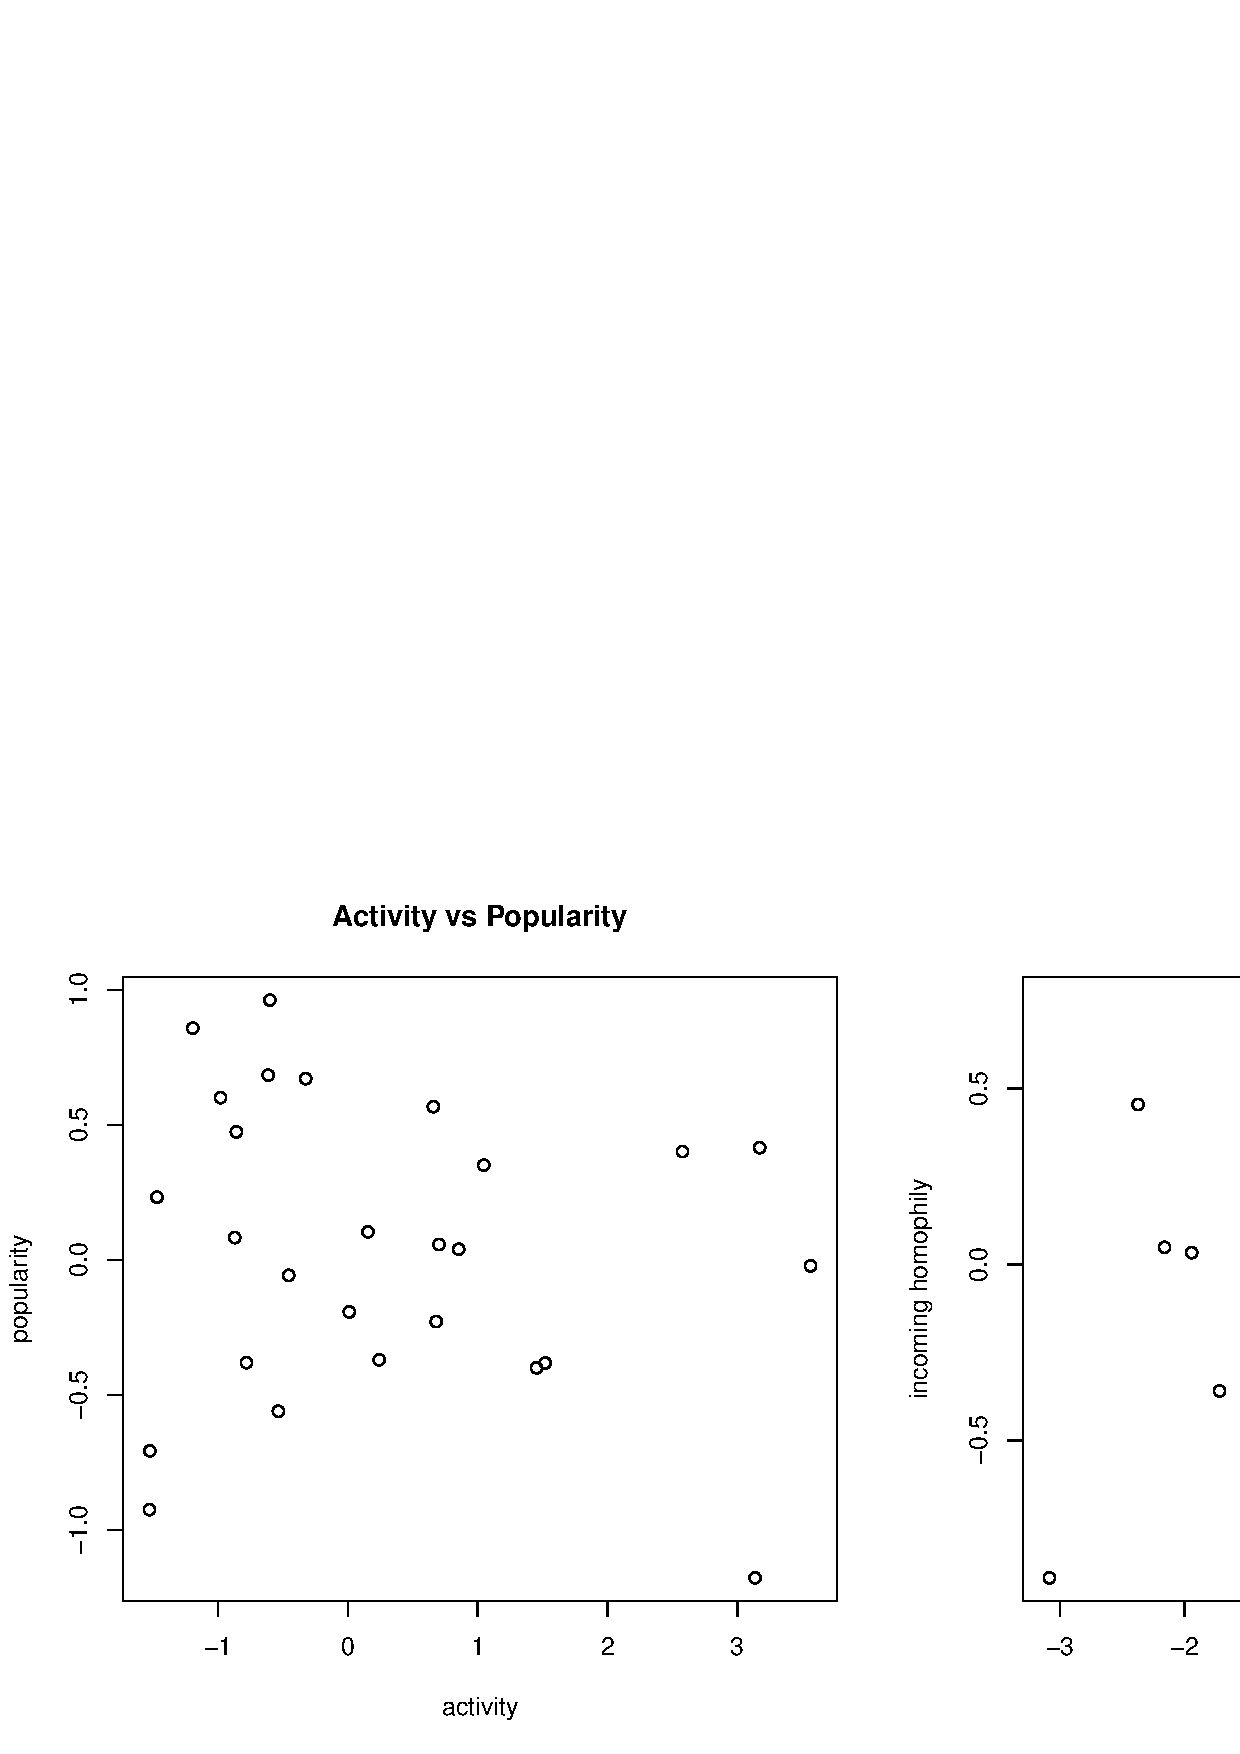
\includegraphics{paper-ranefplotfig2}
\caption{Plots by mixing sender and receiver effects.}
\label{ranefplotfig}
\end{figure}

Note that this also illustrates the big limitation of the cross-effects way of modeling directed networks. We have seperate homophily
effects for incoming ties (match.sex | receiver) and outgoing ties (match.sex | sender). We cannot fit these in one and the same term 
because the sender and receiver groups are modeled as seperate classes. However, we can try to plot them against each other:

\begin{Schunk}
\begin{Sinput}
> par(mfrow = c(1, 2))
> plot(ranef(hansell.2)$sender[, 1], ranef(hansell.2)$receiver[, 
+     1], main = "Activity vs Popularity", xlab = "activity", ylab = "popularity")
> plot(ranef(hansell.2)$sender[, 2], ranef(hansell.2)$receiver[, 
+     2], main = "Homophily", xlab = "outgoing homophily", ylab = "incoming homophily")
\end{Sinput}
\end{Schunk}

Quite interestingly, there seems to be no strong relation between activity and popularity, nor between outgoing and incoming homophily.
This would indicate that the social behaviour of one person towards others is pretty much independent of the social behaviour of the others 
toward this person. 

\subsection{Predicting Random Effects using Cross-level interactions}

Another interesting feature of Mixed Effect models are so called cross-level interactions. In our applications, a cross-level 
interaction is a fixed effect that is an interaction of a dyad attribute and a node attribute. If also the dyad attribute
is a random effect, the cross-level interaction can be interpreted as a preditor of the random effect. \\

An example: suppose we are interested in modeling mutuality:

\begin{Schunk}
\begin{Sinput}
> mutual.1 <- lmergm(hansell ~ edges + mutual + (edges + mutual | 
+     sender) + (edges + mutual | receiver))
> summary(mutual.1)
\end{Sinput}
\begin{Soutput}
Generalized linear mixed model fit by the Laplace approximation 
Formula: y ~ 1 + mutual + (1 + mutual | sender) + (1 + mutual | receiver) 
   Data: cmatrix 
   AIC BIC logLik deviance
 653.6 690 -318.8    637.6
Random effects:
 Groups   Name        Variance Std.Dev. Corr   
 sender   (Intercept) 1.87838  1.37054         
          mutual      0.91135  0.95465  -0.264 
 receiver (Intercept) 0.69032  0.83086         
          mutual      1.59905  1.26454  -0.150 
Number of obs: 702, groups: sender, 27; receiver, 27

Fixed effects:
            Estimate Std. Error z value Pr(>|z|)    
(Intercept)  -2.0865     0.3430  -6.082 1.19e-09 ***
mutual        1.1441     0.4394   2.604  0.00922 ** 
---
Signif. codes:  0 ‘***’ 0.001 ‘**’ 0.01 ‘*’ 0.05 ‘.’ 0.1 ‘ ’ 1 

Correlation of Fixed Effects:
       (Intr)
mutual -0.278
\end{Soutput}
\end{Schunk}
Note first the interpretation of this model is a bit subtle, as we include random effects of mutuality of both the sender and receiver.
The mutual term on the sender level is the effect that measures the tendency of an ego to connect back to an incoming tie from the network.
The mutual term on the receiver level is the effect of the other tie to 'connect back' when an outgoing tie is existent. \\

The model shows that there is quite some variation between the nodes in the effect of mutuality, both at the sender and receiver level. 
Therefore, a followup question might be if gender might have something to do with this variation. We include the cross level interaction of 
the mutuality term and the gender of the receiving node. This automatically includes the marginal term of the gender of the receiving node.
\begin{Schunk}
\begin{Sinput}
> mutual.2 <- lmergm(hansell ~ edges + mutual * nodeifactor("sex") + 
+     (edges + mutual | sender) + (edges + mutual | receiver))
> summary(mutual.2)
\end{Sinput}
\begin{Soutput}
Generalized linear mixed model fit by the Laplace approximation 
Formula: y ~ 1 + mutual * nodeifactor.sex.male + (1 + mutual | sender) +      (1 + mutual | receiver) 
   Data: cmatrix 
   AIC BIC logLik deviance
 648.5 694 -314.3    628.5
Random effects:
 Groups   Name        Variance Std.Dev. Corr   
 sender   (Intercept) 1.91481  1.38377         
          mutual      0.61745  0.78578  -0.403 
 receiver (Intercept) 0.82089  0.90603         
          mutual      0.25898  0.50890  -0.077 
Number of obs: 702, groups: sender, 27; receiver, 27

Fixed effects:
                            Estimate Std. Error z value Pr(>|z|)    
(Intercept)                  -2.2445     0.4159  -5.396 6.80e-08 ***
mutual                        2.2661     0.4516   5.018 5.22e-07 ***
nodeifactor.sex.male          0.2133     0.4365   0.489 0.624974    
mutual:nodeifactor.sex.male  -2.2132     0.6231  -3.552 0.000383 ***
---
Signif. codes:  0 ‘***’ 0.001 ‘**’ 0.01 ‘*’ 0.05 ‘.’ 0.1 ‘ ’ 1 

Correlation of Fixed Effects:
            (Intr) mutual ndfc..
mutual      -0.372              
ndfctr.sx.m -0.528  0.239       
mtl:ndfct..  0.192 -0.627 -0.311
\end{Soutput}
\end{Schunk}
The result is very convincing that gender has a big influence of the importance of mutuality. The cross level interaction effect is very big
and significant, and has reduced the variance of the mutuality term on the receiver level from 1.60 to 0.26. 
We can conclude from these results that girls can expect much greater mutuality than boys.  


\section{A bigger example: The Lazega Data}
\label{section.lazega}

\cite{snijders2006new} present several examples based on a data collection by Lazega,
described extensively in \cite{lazega2001collegial}, on relations between lawyers in a New England law firm (also see \cite{lazega1999multiplexity}).
In this section we take this data and show how mixed effect random graph models reveal properties of a network that might otherwise be hard to discover.
The Lazega data is included in the \texttt{lmergm} package.

\subsection{Lawyer Homophily}

Snijders et al. report significant effects for 'office homophily', 'practice homophily', and a negative effect for the difference in experience.
We start to see if we can find the same thing, by fitting a model that includes these terms, and also a random coefficient for intercept and transitivity:

\begin{Schunk}
\begin{Sinput}
> data(ELfriend36)
> friends <- ELfriend36
> mymodel5 <- lmergm(friends ~ edges + mutual + transitive + match("office") + 
+     match("practice") + absdiff("years") + (edges | sender) + 
+     (edges | receiver))
> summary(mymodel5)
\end{Sinput}
\begin{Soutput}
Generalized linear mixed model fit by the Laplace approximation 
Formula: y ~ 1 + mutual + transitive + nodematch.office + nodematch.practice +      absdiff.years + (1 | sender) + (1 | receiver) 
   Data: cmatrix 
   AIC   BIC logLik deviance
 790.3 831.4 -387.2    774.3
Random effects:
 Groups   Name        Variance Std.Dev.
 sender   (Intercept) 1.02802  1.01391 
 receiver (Intercept) 0.29809  0.54598 
Number of obs: 1260, groups: sender, 36; receiver, 36

Fixed effects:
                   Estimate Std. Error z value Pr(>|z|)    
(Intercept)        -4.18162    0.37465 -11.161  < 2e-16 ***
mutual              2.33710    0.23344  10.012  < 2e-16 ***
transitive          0.17820    0.02433   7.326 2.38e-13 ***
nodematch.office    1.12438    0.25138   4.473 7.72e-06 ***
nodematch.practice  0.39826    0.19646   2.027   0.0426 *  
absdiff.years      -0.03741    0.01654  -2.261   0.0238 *  
---
Signif. codes:  0 ‘***’ 0.001 ‘**’ 0.01 ‘*’ 0.05 ‘.’ 0.1 ‘ ’ 1 

Correlation of Fixed Effects:
            (Intr) mutual trnstv ndmtch.f ndmtch.p
mutual      -0.175                                
transitive  -0.393 -0.072                         
nodmtch.ffc -0.348 -0.110 -0.277                  
ndmtch.prct -0.305 -0.047  0.066  0.068           
absdiff.yrs -0.446  0.053  0.111  0.011   -0.046  
\end{Soutput}
\end{Schunk}

\subsection{More here ...}



\clearpage
\begin{appendices}

\section{The \texttt{lmergm} package}
\label{appendix.package}

Most of the work of this research has gone into the implemention of the code. We decided that it might be helpful to put the functions
that were used into a R package so that others can experiment with it. However, this does not mean that the package is 
considered stable and ready for publication. It is actually in an early stage and has hardly been tested and comes with no guarantees.
Also no documentation has been written yet for any of the functions.

\subsection*{Installation}

To install the package, please first download the latest version of both of its dependencies from CRAN
\begin{verbatim}
install.packages("lme4", repos="http://cran.r-project.org/");
install.packages("ergm", repos="http://cran.r-project.org/");
\end{verbatim}
Next, install the \texttt{lmergm} package:
\begin{verbatim}
install.packages("lmergm", repos="http://www.stat.ucla.edu/~jeroen", type="source");
\end{verbatim}

\subsection*{How to Use}

There are basically 3 functions in the package that are useful to the end user:
\begin{itemize}
\item \texttt{buildcmatrix(formula, verbose)} (returns a matrix)
\item \texttt{ergm2lme4(formula)} (returns a formula)
\item \texttt{lmergm(formula, verbose, ...)} (returns an \texttt{lme4} mer object)
\end{itemize}
All functions need the \texttt{lmergm} formula to do their job. The buildcmatrix function extracts the network terms from the formula, 
and then uses functions in the \texttt{ergm} package to build the matrix with covariates of all the terms in the formula. 
For example, if we could create a formula for the network object that was displayed in figure \ref{fig:mininet1}
\begin{Schunk}
\begin{Sinput}
> buildcmatrix(mininet ~ match("sex") + transitiveties + mutual + 
+     (1 | sender) + (1 | receiver))
\end{Sinput}
\begin{Soutput}
  y nodematch.sex transitiveties mutual receiver sender
1 1             0              0      1        3      2
2 1             1              1      0        1      3
3 0             1              2      1        3      1
4 1             0              1      1        2      3
5 0             0              2      1        1      2
6 1             0              1      0        2      1
\end{Soutput}
\end{Schunk}

The \texttt{ergm2lme4} function takes the same formula and converts it to a valid \texttt{lme4} formula:
\begin{Schunk}
\begin{Sinput}
> ergm2lme4(mininet ~ match("sex") + transitiveties + mutual + 
+     (1 | sender) + (1 | receiver))
\end{Sinput}
\begin{Soutput}
[1] "y ~  nodematch.sex + transitiveties + mutual + (1 | sender) + (1 | receiver)"
\end{Soutput}
\end{Schunk}
It has to do some tricky things to be able to guess the names of the \texttt{ergm} terms, as they will be returned created by \texttt{buildcmatrix}. \\

Finally, \texttt{lmergm} is a user friendly interface to the entire process. It first uses \texttt{buildcmatrix} and \texttt{ergm2lme4}
to generate the appropriate covariates matrix and \texttt{lme4} formula. Then it calls \texttt{glmer} using the just generated objects and sets
\texttt{family="binomial"}. Furthermore, it passes anything in the elipse (...) on to the \texttt{glmer} function. 

\begin{Schunk}
\begin{Sinput}
> mymodel <- lmergm(mininet ~ match("sex") + transitiveties + mutual + 
+     (1 | sender) + (1 | receiver), verbose = T)
\end{Sinput}
\begin{Soutput}
Building covariates matrix...
Compressed MPLE covariate matrix has 6 rows.
Converting formula...
y ~  nodematch.sex + transitiveties + mutual + (1 | sender) + (1 | receiver) 
Calling lme4...
  0: 1.1429253e-09:  1.15470  1.15470  71.4107 -0.662521 -46.4807 -2.05432
  1: 1.1429253e-09:  1.15470  1.15470  71.4107 -0.662521 -46.4807 -2.05432
\end{Soutput}
\end{Schunk}

\section{Code to reproduce results, tables and figures}
\label{appendix.code}

\begin{verbatim}

library(lmergm);
library(xtable);
data(hansell);

#Directed 3 node network
mininet <- network(matrix(c(0,0,1,1,0,1,0,1,0),3), directed=T, 
  vertex.attr=list(sex=c("M","F","M")));
par(mar=c(0,0,0,0))
plot(mininet, edge.lwd=5, vertex.cex=5, arrowhead.cex=3, vertex.col="sex", 
  displaylabels=T, label.cex=2)


mydata <- abs(buildcmatrix(mininet ~ match("sex") + transitiveties));
print(xtable(mydata, digits=0, caption = "Full expansion of the directed 3 node network.", 
  label="minitable"));
	
#Undireced 3 node network	
mininet2 <- network(matrix(c(0,0,1,1,0,1,0,1,0),3), directed=F, 
	vertex.attr=list(sex=c("M","F","M")));
par(mar=c(0,0,0,0))
plot(mininet2, edge.lwd=5, vertex.cex=5, arrowhead.cex=3, vertex.col="sex", 
  displaylabels=T, label.cex=2)	
	
mydata <- abs(buildcmatrix(mininet ~ match("sex")))[c(6,4,3),];
names(mydata)[3:4] <- c("node", "node")
print(xtable(mydata, digits=0, caption = "Full expansion of an undirected 3 node network.", 
  label="minitable2"));	

#Coefficient Histograms:	
hansell.ca1 <- ergm(hansell ~ receiver(0));
hansell.ca2 <- ergm(hansell ~ sender(0));
par(mfrow=c(1,2));
hist(coef(hansell.ca1), main="receiver", xlab="mle");
hist(coef(hansell.ca2), main="sender", xlab="mle");

#Coefficient plots:
hansell.cb1 <- lmergm(hansell ~ edges + (1|receiver))
hansell.cb2 <- lmergm(hansell ~ edges + (1|sender))
par(mfrow=c(1,2));
plot(coef(hansell.ca1), coef(hansell.cb1)$receiver[[1]], main="receiver", 
  xlab="Fixed coefficients", ylab="Random BLUPS", xlim=c(-3,1), ylim=c(-3,1))
abline(0,1, col="red")
plot(coef(hansell.ca2), coef(hansell.cb2)$sender[[1]], main="sender", 
  xlab="Fixed coefficients", ylab="Random BLUPS", xlim=c(-3,1), ylim=c(-3,1))
abline(0,1, col="red")
	
#shrinkage table:
allcoef <- data.frame("popularity.fixed"= coef(hansell.ca1), 
  "popularity.random"=coef(hansell.cb1)$receiver[[1]], 
  "activity.fixed" = coef(hansell.ca2), "activity.random" = coef(hansell.cb2)$sender[[1]]);
print(xtable(allcoef, caption = "Fixed effect MLE's and random effect BLUPs of popularity 
  and activity", label="coeftable", align=c("lrrrr")));
  
#Hansell M0  
hansell.0 <- ergm(hansell ~ edges + transitiveties + match('sex'), MPLEonly=T);
summary(hansell.0);

#Hansell M1
hansell.1 <- lmergm(hansell ~ edges + transitiveties + match('sex') + 
  (edges | sender) + (edges | receiver));
summary(hansell.1);

#Hansell M2
hansell.2 <- lmergm(hansell ~ edges + transitiveties + match('sex') + 
  (edges + match('sex') | sender) + (edges  + match("sex") | receiver));
summary(hansell.2);

#Table with M0-M2 coefficients
allmodels <- list(hansell.0, hansell.1, hansell.2);
mytable <- as.data.frame(cbind(M0=coef(hansell.0),M1=fixef(hansell.1), M2=fixef(hansell.2)));
mytable[c("u0","u2","u12"),] <- NA;
mytable[c("v0","v2","v12"),] <- NA;
mytable["AIC",] <- sapply(allmodels, AIC);
mytable["BIC",] <- sapply(allmodels, BIC);
mytable["Deviance",] <- -2*sapply(allmodels, logLik);
mytable["u0", "M1"] <- VarCorr(hansell.1)$sender[1,1];
mytable["u0", "M2"] <- VarCorr(hansell.2)$sender[1,1];
mytable["v0", "M1"] <- VarCorr(hansell.1)$receiver[1,1];
mytable["v0", "M2"] <- VarCorr(hansell.2)$receiver[1,1];
mytable["u2", "M2"] <- VarCorr(hansell.2)$sender[2,2];
mytable["v2", "M2"] <- VarCorr(hansell.2)$receiver[2,2];
mytable["u12", "M2"] <- VarCorr(hansell.2)$sender[1,2];
mytable["v12", "M2"] <- VarCorr(hansell.2)$receiver[1,2];
rownames(mytable) <- c("$\\beta_0$","$\\beta_1$","$\\beta_2$",
  "$\\upsilon_0$","$\\upsilon_2$","$\\upsilon_{02}$",
  "$\\nu_0$","$\\nu_2$","$\\nu_{02}$",
  "AIC", "BIC", "Deviance");
print(xtable(mytable, caption = "Model Coefficients for Hansell data.", 
  label="hansellcoef", align=c("lrrr")),sanitize.rownames.function = I, 
  hline=c(-1,0,3,9,nrow(mytable)));

#random effect plots
par(mfrow=c(1,2))
plot(ranef(hansell.2)$sender, main="Sender", xlab="homophily", ylab="activity")
plot(ranef(hansell.2)$receiver, main="Receiver", xlab="homophily", ylab="popularity")

#more random effect plots
par(mfrow=c(1,2))
plot(ranef(hansell.2)$sender[,1], ranef(hansell.2)$receiver[,1], 
  main="Activity vs Popularity", xlab="activity", ylab="popularity");
plot(ranef(hansell.2)$sender[,2], ranef(hansell.2)$receiver[,2], 
  main="Homophily", xlab="outgoing homophily", ylab="incoming homophily");

#mutuality example model 1
mutual.1 <- lmergm(hansell ~ edges + mutual + (edges + mutual | sender) + 
  (edges + mutual | receiver));  
summary(mutual.1);

#mutuality example model 2
mutual.2 <- lmergm(hansell ~ edges + mutual * nodeifactor("sex") + 
  (edges + mutual | sender) + (edges + mutual | receiver))
summary(mutual.2)  

\end{verbatim}



\end{appendices}

\bibliographystyle{apalike}	% (uses file "plain.bst")
\bibliography{paper}
	
\end{document}
